\fancyhead[C]{\normalsize\textbf{$\qquad$ Teil II: Multiple-Choice}}
\section*{Aufgabe 2 (32 Punkte)}
\vspace{0.4cm}
\subsection*{\frage{1}{3}}
Welcher der folgenden mathematischen Ausdrücke beschreibt das nachfolgende Problem:
\begin{displayquote}
	Finde den Punkt $P = (x,y)$ auf der Hyperbel $x^2 - 9 y^2 = 16$ mit dem kleinsten
	Abstand zum Punkt $P_0 = (0,-3)$.
\end{displayquote}
\renewcommand{\labelenumi}{(\alph{enumi})}
\begin{enumerate}
	\item 
	$\min_{x,y} D(x,y) = x^2 - 9y^2 - 16$ so, dass
	$\sqrt{x^2 + (y-3)^2} = 0$.
	\item 
	$\min_{x,y} D(x,y) = \sqrt{x^2 + ( y + 3)^2}$ so, dass
	$x^2 - 9 y^2 - 16  = 0$.
	\item 
	$\max_{x,y} D(x,y) = 16 - x^2 + 9y^2 $ so, dass
	$\sqrt{x^2 + (y+3)^2} = 0$.
	\item 
	$\min_{x,y} D(x,y) = \sqrt{x^2 + ( y - 3)^2}$ so, dass
	$x^2 - 9 y^2 - 16  = 0$.
	\item 
	$\min_{x,y} D(x,y) = x^2 - 9y^2 - 16$ so, dass
	$\sqrt{x^2 + (y+3)^2} = 0$.
	\item
	$\max_{x,y} D(x,y) = \sqrt{x^2 + ( y - 3)^2}$ so, dass
	$x^2 - 9 y^2 - 16  = 0$.
\end{enumerate}
\ \\
\textbf{Lösung:}
\begin{mdframed}
\underline{\textbf{Vorgehensweise:}}
\renewcommand{\labelenumi}{\theenumi.}
\begin{enumerate}
\item Verwende die Distanz zwischen zwei Punkten.
\end{enumerate}
\end{mdframed}

\underline{1. Verwende die Distanz zwischen zwei Punkten}\\
Die Distanz von einem Punkt $P=(x,y)$ zu dem Punkt $P_0 = (0,-3)$ ist gegeben durch
die Funktion
\begin{align*}
	D(x,y) = \sqrt{(x-x_0)^2 + (y-y_0)^2}
	=
	 \sqrt{(x-0)^2 + (y-(-3))^2}
	=
	\sqrt{x^2 + (y+3)^2}.
\end{align*}
Das ist die Zielfunktion, welche man versucht zu minimieren. Hiermit bleibt die Antwort (b) übrig. 
Die Nebenbedingung 
\begin{align*}
	x_2 - 9y^2  - 16  = 0 
	\ \Leftrightarrow \
	x^2 -9y^2 = 16
\end{align*}
entspricht der Forderung, dass $(x,y) $ auf der Hyperbel liegen muss.\\
\\
Damit ist Antwort(b) korrekt.
\begin{center}
	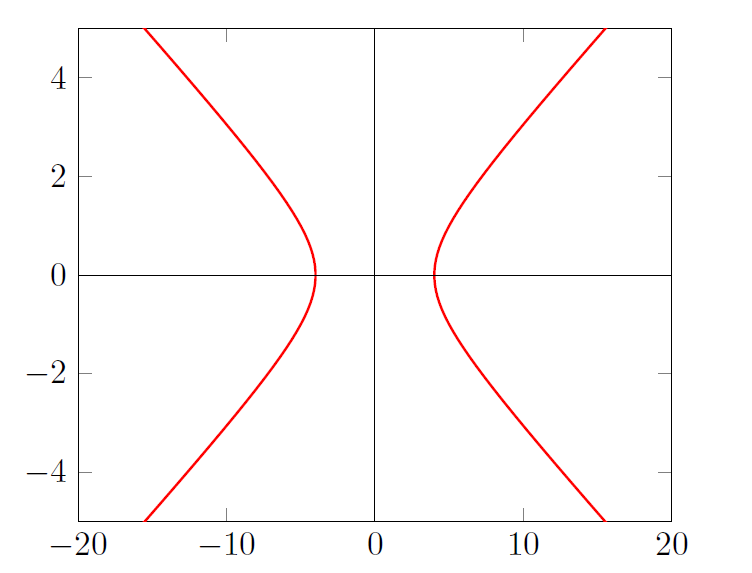
\includegraphics[width=0.6\textwidth]{pictures/aufgabe2_1_1}
\end{center}

\newpage

\subsection*{\frage{2}{4}}
Sei $ f \ : \ D_f \to \mathbb{R} $ eine ungerade Funktion zweier reellen Variablen, d.h., $f(x,y) = - f(-x,-y)$ für alle $(x,y) \in D_f$, mit einem lokalen Maximum, welches nicht am Nullpunkt $(0,0)$ liegt.\\
\\ 
Welche der folgenden Aussagen ist korrekt?
\renewcommand{\labelenumi}{(\alph{enumi})}
\begin{enumerate}
	\item Die Funktion $f$ hat mindestens ein lokales Minimum.
	\item Die Funktion $f$ hat mindestens einen Sattelpunkt.
	\item Die Funktion $f$ hat mindestens zwei lokale Maxima.
	\item Die Funktion $f$ hat mindestens ein globales Maximum.
	\item Die Funktion $f$ hat kein globales Maximum.
\end{enumerate}
\ \\
\textbf{Lösung:}
\begin{mdframed}
	\underline{\textbf{Vorgehensweise:}}
	\renewcommand{\labelenumi}{\theenumi.}
	\begin{enumerate}
		\item Verwende Umgebungen, um die korrekte Antwort zu finden.
	\end{enumerate}
\end{mdframed}
\underline{1. Verwende Umgebungen, um die korrekte Antwort zu finden}\\
Uns ist bekannt, dass die ungerade Funktion $f$ ein lokales Maximum $P_0 = (x_0,y_0) \neq (0,0)$ besitzt. 
Da $f$ ungerade ist, liegt die Vermutung nahe, dass $Q_0 = (-x_0, -y_0)$ ein lokales Minimum ist.\\
\\
Dies werden wir nun zeigen: Da $(x_0,y_0)$ ein Maximum von $f$ ist, existiert eine Umgebung $U_{(x_0,y_0)}$ um den Punkt $P_0$, sodass
\begin{align*}
	f(x,y) \leq f(x_0,y_0)
\end{align*}
für alle $(x,y) \in  U_{(x_0,y_0)}$ gilt.\\
Anschauliche Vorstellung einer Umgebung um einen Punkt $P$: 
Kreisscheibe mit Mittelpunkt $P$ und hinreichend kleinem Radius.\\
Die Menge
\begin{align*}
	U_{(-x_0,-y_0)} 
	= \{
		(x,y) \in \mathbb{R}^2 \ | (-x,-y) \in U 
	\}
\end{align*}
ist eine Umgebung um den Punkt $Q_0 = (-x_0,-y_0)$.
Für ein beliebiges $(x,y) \in U_{(-x_0,-y_0)}  $ erhalten wir
\begin{align*}
	f(\underbrace{-x,-y}_{  \in U_{(x_0,y_0) }}) \leq f(x_0, y_0). 
\end{align*}
Weiter gelten aufgrund der Punktsymmetrie:
\begin{align*}
	f(x_0, y_0) &= - f(\underbrace{-x_0,-y_0}_{ \in U_{(-x_0,-y_0) }})\\
	f(-x,-y)  &= -f(x,y).
\end{align*}
Eingesetzt in die Ungleichung liefert dies:
\begin{align*}
	-f(x,y) \leq - f(-x_0, -y_0)
	\ \Leftrightarrow \
	f(x,y) \geq f(-x_0,-y_0).
\end{align*}
Da die Ungleichung für ein beliebiges $(x,y) \in U_{(-x_0,-y_0)} $ gilt, liegt in $(-x_0,-y_0)$ eine lokales Minimum vor.\\
\\
Damit ist die Antwort (a) korrekt. Alternativ lassen sich für (b) - (e) auch Gegenbeispiele finden.

\newpage
\subsection*{\frage{3}{3}}
Sei $f$ eine stetige reellwertige Funktion auf einem abgeschlossenen Intervall $[a,b]$.\\
\\
Was ist eine der Aussagen des Hauptsatzes der Differential- und Integralrechnung?
\renewcommand{\labelenumi}{(\alph{enumi})}
\begin{enumerate}
	\item 
	$\int_{-\infty}^b f(x) \ dx = 
	\lim_{a \to -\infty} \int_{a}^b f(x) \ dx
	$.
	\item 
	$\int f(g(x)) g^\prime(x) \ dx
	= \int f(y) \ d(y)
	= F(g(x) ) + C
	$, wobei $F$ eine beliebige Stammfunktion von $f$ ist.
	\item 
	$\int u(x) v^\prime(x) \ dx = u(x) v(x)  - \int u^\prime(x) v(x) \ dx$.
	\item 
	$\int_a^b f(x) \ dx
	=\left[F(x)\right]_a^b= F(b) +F(a)
	$, wobei $F$ eine beliebige Stammfunktion von $f$ ist.
	\item 
	Sei die Funktion $F$ definiert als $F(x) = \int_a^x f(u) \ du$.
	Dann ist $F$ eine Stammfunktion von $f$.
\end{enumerate}
\ \\
\textbf{Lösung:}
\begin{mdframed}
\underline{\textbf{Vorgehensweise:}}
\renewcommand{\labelenumi}{\theenumi.}
\begin{enumerate}
\item Rufe dir den Hauptsatzes der Differential- und Integralrechnung in Erinnerung.
\end{enumerate}
\end{mdframed}

\underline{1. Rufe dir den Hauptsatzes der Differential- und Integralrechnung in Erinnerung}\\
Der Hauptsatz unterteilt sich in zwei Teile:
\begin{enumerate}
	\item[1.] 
	Sei $I \subset \mathbb{R}  $ ein Intervall und $f : I \to \mathbb{R}$ stetig.
	Dann ist
	\begin{align*}
		F : I \to \mathbb{R}, \quad F(x) = \int \limits_{c}^x f(u) \ du
	\end{align*}
	für jedes $c \in I $ eine Stammfunktion von $f$ ($F^\prime = f$).
	\item[2.]
	Sei $I = [a,b] \subset \mathbb{R} $ ein Intervall und $f: I \to \mathbb{R}$ stetig mit zugehöriger Stammfunktion $F : I \to \mathbb{R}$. Dann gilt
	\begin{align*}
		\int \limits_a^b f(x) \ dx = F(b) - F(a).
	\end{align*}
\end{enumerate}
Da die Antwort (e) dem ersten Teil des Hauptsatzes entspricht, ist diese Antwort korrekt.\\
\\
Die Antwortmöglichkeit (a) entspricht der Definition eines uneigentlichen Integrals.
Durch (b) wird die Integration durch Substitution definiert. Antwort (c) entspricht der partiellen Integration. 
Die Möglichkeit (d) ist falsch (siehe zweiter Teil des Hauptsatzes). 


\newpage

\subsection*{\frage{4}{3}}
Sei $ f $ eine gerade Funktion.
Für $a > 0$ ist $\int_{-a}^a f(x) \ dx$ gleich:
\renewcommand{\labelenumi}{(\alph{enumi})}
\begin{enumerate}
	\item 
	$ 0 $.
	\item
	$ 2 \int_a^0 f(x) \ dx $.
	\item
	$ -2  \int_a^0 f(x) \ dx$.
	\item
	$ 1 $.
	\item
	Keine der obigen Antworten ist korrekt.
\end{enumerate}
\ \\
\textbf{Lösung:}
\begin{mdframed}
\underline{\textbf{Vorgehensweise:}}
\renewcommand{\labelenumi}{\theenumi.}
\begin{enumerate}
\item Nutze die Eigenschaft der geraden Funktion.
\end{enumerate}
\end{mdframed}

\underline{1. Nutze die Eigenschaft der geraden Funktion }\\
Da $f$ eine gerade Funktion ist, gilt $f(x) = f(-x)$ für alle $x \in D_f$.
Mit der Substitution $y = -x $ erhalten wir zunächst.
\begin{align*}
	\frac{dy}{dx} = -1 
	\ \Leftrightarrow \
	dx = - dy
\end{align*}
Damit gilt:
\begin{align*}
	\int \limits_{- a}^a f(x) \ dx
	&=
	\int \limits_{-a}^0 f(x) \ dx
	+ 
	\int \limits_{0}^a f(x) \ dx
	=
	\int \limits_{-a}^0 f(-x) \ dx
	+ 
	\int \limits_{0}^a f(x) \ dx\\
	&=
	\int \limits_{a}^0 -f(y) \ dy
	+ 
	\int \limits_{0}^a f(x) \ dx
	=
	-\int \limits_{a}^0 f(y) \ dy
	+ 
	\int \limits_{0}^a f(x) \ dx\\
	&=
	-\int \limits_{a}^0 f(x) \ dy
	- 
	\int \limits_{a}^0 f(x) \ dx
	= 
	-2 
	\int \limits_{a}^0 f(x) \ dx.
\end{align*}
Dabei haben wir auch verwendet, dass bei Vertauschen der Integrationsgrenzen das Vorzeichen wechselt.

Somit ist Antwort (c) korrekt.\\
\\
Die schnellere Variante ist:
Da $f$ gerade (also achsensymmetrisch) ist, folgt durch Vertauschen der Integrationsgrenzen
\begin{align*}
	\int \limits_{- a}^a f(x) \ dx
	=
	2 \int \limits_{0}^a f(x) \ dx
	= 
	- 2 \int \limits_{a}^0 f(x) \ dx.
\end{align*}


\newpage
\subsection*{\frage{5}{4}}
$A$ ist eine $(m \times n)$-dimensionale und invertierbare Matrix mit $m,n \in \mathbb{N}$.\\
\\
Es folgt:
\renewcommand{\labelenumi}{(\alph{enumi})}
\begin{enumerate}
	\item 
	Der Rang von $A$ ist $\mathrm{rg}(A) = m < n$.
	\item 
	Wenn $A$ eine Diagonalmatrix ist, dann gilt $\det(A) = \det(A^{-1})$.
	\item 
	Wenn $A$ eine idempotente Matrix ist, d.h. $A = A^2$, dann gilt $\det(A) = 1$.
	\item 
	Es existiert ein Vektor $\mathbf{x} \neq 0$ so, dass $A \mathbf{x} = 0$.
	\item 
	$A$ ist nicht symmetrisch  für $m=n$. 
\end{enumerate}
\ \\
\textbf{Lösung:}
\begin{mdframed}
\underline{\textbf{Vorgehensweise:}}
\renewcommand{\labelenumi}{\theenumi.}
\begin{enumerate}
\item Schließe falsche Antworten aus.
\end{enumerate}
\end{mdframed}

\underline{1. Schließe falsche Antworten aus}\\
Da die Matrix $A$ invertierbar ist, muss $A$ eine quadratische Matrix mit vollem Rang sein, d.h. $\mathrm{rg}(A) = m= n$. Somit kann Antwort (a) nicht gelten.
Aufgrund der Invertierbarkeit besitzt die Gleichung
\begin{align*}
	A \mathbf{x} = 0
\end{align*} 
nur die Lösung $\mathbf{x} = 0$. Damit kann Möglichkeit (d) nicht gelten.
Wegen 
\begin{align*}
	\det(A^{-1}) = \frac{1}{\det(A)}
\end{align*}
gilt $\det(A) = \det(A^{-1})$ nur für die Diagonalmatrix $A = I$ (und nicht für die anderen Diagonalmatrizen). Dies ist ein Gegenbeispiel zu (b).\\
Da $A$ invertierbar ist, ist uns $n = m$ bekannt. Hieraus können wir jedoch keine Rückschlüsse auf die Symmetrie ziehen. Deswegen fällt Antwort (e) auch weg.\\
\\
Übrig bleibt die Möglichkeit (c). In der Tat folgt aus der Idempotenz von $A$:
\begin{align*}
	A = A^2 
	\ \Rightarrow \
	\det(A) = \det(A^2) = \det(A) \det(A).
\end{align*}
Diese Gleichung ist für $\det(A) = 0$ und $\det(A) = 1$ erfüllt.
Aufgrund der Invertierbarkeit von $A$ ist nur $\det(A) = 1$ möglich. \\
\\
Also ist Antwort (c) korrekt.




\newpage

\subsection*{\frage{6}{3}}
Sei $\mathbf{u} $ ein Eigenvektor einer Matrix $A$ mit zugehörigem Eigenwert $\lambda$.
\\
Es folgt, dass 
\begin{align*}
	AA \mathbf{u}
\end{align*}
gleich:
\renewcommand{\labelenumi}{(\alph{enumi})}
\begin{enumerate}
	\item 
	$ \frac{1}{\lambda} \mathbf{u} $ ist.
	\item 
	$ \lambda \mathbf{u} $ ist.
	\item
	$ \lambda^2 \mathbf{u}$ ist.
	\item
	$ 2\lambda \mathbf{u} $ ist.
	\item 
	$ \lambda \mathbf{u}^2 $ ist.
\end{enumerate}
\ \\
\textbf{Lösung:}
\begin{mdframed}
\underline{\textbf{Vorgehensweise:}}
\renewcommand{\labelenumi}{\theenumi.}
\begin{enumerate}
\item Verwende die Definition des Eigenvektors.
\end{enumerate}
\end{mdframed}

\underline{1. Verwende die Definition des Eigenvektors}\\
Ein Vektor $\mathbf{u} \neq 0$ heißt Eigenvektor einer quadratischen Matrix $A$ zum Eigenwert $\lambda$, falls
\begin{align*}
	A \mathbf{u} = \lambda \mathbf{u}
\end{align*}
gilt.\\
\\
$\mathbf{u}$ ist ein Eigenvektor der Matrix $A$ mit Eigenwert $\lambda $.
Somit folgt:
\begin{align*}
	A A \mathbf{u} 
	=
	A \lambda \mathbf{u} 
	= 
	\lambda A \mathbf{u} 
	= 
	\lambda \lambda \mathbf{u}
	= 
	\lambda^2 \mathbf{u}.
\end{align*}
Damit ist Antwort (c) korrekt.



\newpage
\subsection*{\frage{7}{3}}
Seien $A$ und $B$ zwei reguläre $(n \times n)$-dimensionale Matrizen mit $\det(A) = \det(B) = n$.\\
Es folgt, dass $\det(2AA^{-1} B B^{-1} B A)$:
\renewcommand{\labelenumi}{(\alph{enumi})}
\begin{enumerate}
	\item 
	gleich $0$ ist.
	\item
	gleich $6n$ ist.
	\item
	gleich $n^6$ ist.
	\item
	gleich $2 n^2$ ist.
	\item
	gleich $2^n n^2$ ist.
\end{enumerate}
\ \\
\textbf{Lösung:}
\begin{mdframed}
\underline{\textbf{Vorgehensweise:}}
\renewcommand{\labelenumi}{\theenumi.}
\begin{enumerate}
\item Verwende die Rechenregeln für Determinanten.
\end{enumerate}
\end{mdframed}

\underline{1. Verwende die Rechenregeln für Determinanten}\\
Die korrekte Antwort erhalten wir, indem wir zunächst den Ausdruck innerhalb der Determinante vereinfachen. 
Darauf folgend verwenden wir die Rechenregeln
\begin{align*}
	\det(c A)&= c^n \det(A)\\
	\det(AB) &= \det(A) \det(B).
\end{align*}
Hiermit erhalten wir:
\begin{align*}
	\det(2AA^{-1} B B^{-1} B A)
	=
	\det(2I I B A)
	=
	\det(2B A)
	=
	2^n \det(BA) 
	=
	2^n \det(B) \det(A)
	=
	2^n n^2.
\end{align*}
Damit ist Antwort (d) korrekt.

\newpage

\subsection*{\frage{8}{3}}
Sei $ A $ eine $ (3 \times 1) $-Matrix mit $A = (a_1, a_2, a_3)^\top$, wobei $ a_i \in \mathbb{R}, \ i = 1,2,3$.\\
\\
Sei $ B $ eine $ (3 \times 1) $-Matrix mit $B = (b_1, b_2, b_3)^\top$, wobei $ b_i \in \mathbb{R}, \ i = 1,2,3$.\\
\\
Sei $ C $ eine $ (3 \times 1) $-Matrix mit $C = (c_1, c_2, c_3)^\top$, wobei $ c_i \in \mathbb{R}, \ i = 1,2,3$.\\

Wir definieren die Matrix $D$ durch die folgende Zusammensetzung der Spalten von $A$, $B$ und $C$:
\begin{align*}
	D = [A,B,C]
\end{align*}
Es folgt, dass:
\renewcommand{\labelenumi}{(\alph{enumi})}
\begin{enumerate}
	\item 
	$ \mathrm{rg}(D) = 3 $, wenn $a_1 = a_2$, $b_1 = b_2$ und $c_1 = c_2$.
	\item
	$ \mathrm{rg}(D) = 1 $, wenn $ a_i = 0 $ für alle $ i \in \{1,2,3\} $.
	\item
	$ \mathrm{rg}(D) \geq  2 $, wenn $ a_i \neq 0 $ für mindestens ein $ i \in \{1,2,3\} $.
	\item
	$ \mathrm{rg}(D) < 3 $, wenn $a_3 = 0$, $b_3 = 0$ und $a_1 b_2 = a_2 b_1$. 
	\item
	$ \mathrm{rg}(D) = 2 $, wenn $a_1 = a_2$, $b_1 = b_2$ und $c_1 = c_2$.
	\item 
	Keine der obigen Antworten ist korrekt.
\end{enumerate}
\ \\
\textbf{Lösung:}
\begin{mdframed}
\underline{\textbf{Vorgehensweise:}}
\renewcommand{\labelenumi}{\theenumi.}
\begin{enumerate}
\item Schließe falsche Antworten aus.
\end{enumerate}
\end{mdframed}

\underline{1. Schließe falsche Antworten aus}\\
Für die Antwort (a), (b), (c) und (e) können wir Gegenbeispiele angeben:
\begin{align*}
	D_a = D_c = D_e
	&=
	\begin{pmatrix}
		1 & 1  & 1\\
		1 & 1 & 1\\
		0 & 0 & 0
	\end{pmatrix}
	\ \Rightarrow \
	\mathrm{rg}(D_a) = \mathrm{rg}(D_c) = \mathrm{rg}(D_e) = 1\\
	D_b
	&=
	\begin{pmatrix}
		0 & 1  & 0 \\
		0 & 0 & 1\\
		0 & 0 & 0
	\end{pmatrix}
	\ \Rightarrow \
	\mathrm{rg}(D_b) = 2
\end{align*}
Die Spalten von links nach rechts sind $A$, $B$ und $C$. Die Indizes dienen nur dazu, dass entsprechende Gegenbeispiel zu kennzeichnen.\\
\\
Offen sind noch die Antwortmöglichkeiten (d) und (f). 
Falls $a_3 = 0 $ und $b_3 = 0 $ ist, können wir die Determinante von $D$ folgend berechnen:
\begin{align*}
	\det(D) = c_3 a_1 b_2 - c_3 a_2 b_1
	= c_3 ( a_1 b_2 - a_2 b_1).
\end{align*}
Gilt zusätzlich $a_1 b_2 = a_2 b_1$, folgt $\det(D) = 0$. Damit ist $D$ nicht invertierbar und es gilt $\mathrm{rg}(D) < 3$.\\
\\
Damit ist Antwort (d) korrekt.



\newpage
\subsection*{\frage{9}{3}}
Sei $ A $ eine $ (5 \times 3) $-dimensionale Matrix mit Rang $ 2 $ und $ B $ eine andere Matrix mit den Dimensionen $ (5 \times 2) $ mit Rang $ 2 $.\\
\\
Wir definieren die Matrix $ C $ durch die folgende Zusammensetzung der Spalten von $ A $ und $ B $:
\begin{align*}
	C = [A, B].
\end{align*}
Es folgt:
\renewcommand{\labelenumi}{(\alph{enumi})}
\begin{enumerate}
	\item 
	$ \det(C) = 4$.
	\item
	$ \mathrm{rg}(C) < 4 $.
	\item
	$ C$ hat vollen Rang.
	\item
	Die Inverse von $C$ existiert nicht.
	\item
	$\det(C) = \det(A) \det(B)$.
\end{enumerate}
\ \\
\textbf{Lösung:}
\begin{mdframed}
	\underline{\textbf{Vorgehensweise:}}
	\renewcommand{\labelenumi}{\theenumi.}
	\begin{enumerate}
		\item Verwende die Definition des Ranges.
	\end{enumerate}
\end{mdframed}

\underline{1. Verwende die Definition des Ranges}\\
Der Rang der Matrix $C$ entspricht der Anzahl der linear unabhängigen Spalten von $C$.
Die Matrix $C$ setzt sich aus den Spalten der Matrix $A$ und $B$ zusammen:
\begin{align*}
	C = [A, B] = [ \mathbf{a}_1, \mathbf{a}_2, \mathbf{a}_3,  \mathbf{b}_1, \mathbf{b}_2 ].
\end{align*}
Hierbei sind $\mathbf{a}_1$, $\mathbf{a}_2$ und $\mathbf{a}_3$ die Spalten von $A$ bzw. $\mathbf{b}_1$ und $\mathbf{b}_2$ die Spalten von $ B$.\\
Wegen $\mathrm{rg}(A) = 2$ sind die Spalten von $A$ linear abhängig. Genauer wissen wir, dass zwei (beliebige) Spalten von $A$ linear unabhängig sind. 
Mit $\mathrm{rg}(B) = 2$ folgt $\mathrm{rg}(C) \leq 4 < 5$.
Damit besitzt keinen vollen Rang und ist deswegen auch nicht invertierbar ((a) und (c) kann somit nicht sein).\\
\\
Somit ist Antwort (d) korrekt.\\
\\
Alternativ lassen sich die restlichen Antworten auch leicht ausschließen:
Wegen $\mathrm{rg}(B) = 2$ kann $\mathrm{rg}(C) $ maximal $4$ sein, d.h. $\mathrm{rg}(C) \leq 4$. Möglichkeit (b) ist somit falsch.
Die letzte Möglichkeit ist nicht definiert, da die Determinante nur für quadratische Matrizen definiert ist.



\newpage
\subsection*{\frage{10}{3}}
Sei $A$ eine $(n \times n)$-dimensionale, nicht-invertierbare Matrix.\\
\\
Welche der folgenden Aussagen trifft auf die Matrix $A$ zu?
\renewcommand{\labelenumi}{(\alph{enumi})}
\begin{enumerate}
	\item 
	$A$ muss negative Eigenwerte haben.
	\item
	Alle Eigenwerte sind positiv.
	\item
	$\det(A)$ ist negativ.
	\item
	$0$ ist ein Eigenwert von $A$.
	\item 
	$\lambda_1 \cdot \lambda_2 \cdot \dots \cdot \lambda_n > 0 $, wobei $\lambda_i$ für $i = 1,2,\dots,n$ die Eigenwerte von $A$ sind.
\end{enumerate}
\ \\
\textbf{Lösung:}
\begin{mdframed}
	\underline{\textbf{Vorgehensweise:}}
	\renewcommand{\labelenumi}{\theenumi.}
	\begin{enumerate}
		\item Nutze den Zusammenhang der Determinante zu den Eigenwerten.
	\end{enumerate}
\end{mdframed}

\underline{1. Nutze den Zusammenhang der Determinante zu den Eigenwerten}\\
Die quadratische Matrix $A$ ist nicht invertierbar. Deswegen gilt
\begin{align*}
	\det(A) = \prod \limits_{i=1}^n \lambda_i = 0.
\end{align*}
Hierbei sind $\lambda_i$ für $i = 1, ..., n$ die Eigenwerte von $A$. Diese sind nicht notwendigerweise verschieden.
Da $\det(A) = 0$ muss mindestens einer dieser Eigenwerte $0$ sein. \\
\\
Damit ist Antwort (d) korrekt.\\
\\
Für Antwort (a) ist
\begin{align*}
	A = 
	\begin{pmatrix}
		1 & 0\\
		0 & 0
	\end{pmatrix}
\end{align*}
ein Gegenbeispiel. Antwort (b),(c) und (e) widerspricht $\det(A) = 0$.
 